%----------------------------------------------------------------------------
\chapter{Háttérismeretek}
%----------------------------------------------------------------------------
Ebben a fejezetben a feladat megértéséhez szükséges technológiákat mutatom be röviden. 

%----------------------------------------------------------------------------
\section{Metamodellezés}
%----------------------------------------------------------------------------

%----------------------------------------------------------------------------
\section{Virtuális gépek}
%----------------------------------------------------------------------------

%----------------------------------------------------------------------------
\section{Peer-to-peer fájlátvitel}
%----------------------------------------------------------------------------
A Peer-to-Peer(P2P) hálózat olyan, aminek a csomópontjai nem egy kitüntetett géppel 
kommunikálnak, hanem közvetlenül egymással. A klasszikus kliens-szerver és a P2P hálózat felépítését
a következő ábrák szemléltetik:

\begin{figure}[!ht]
	\centering
	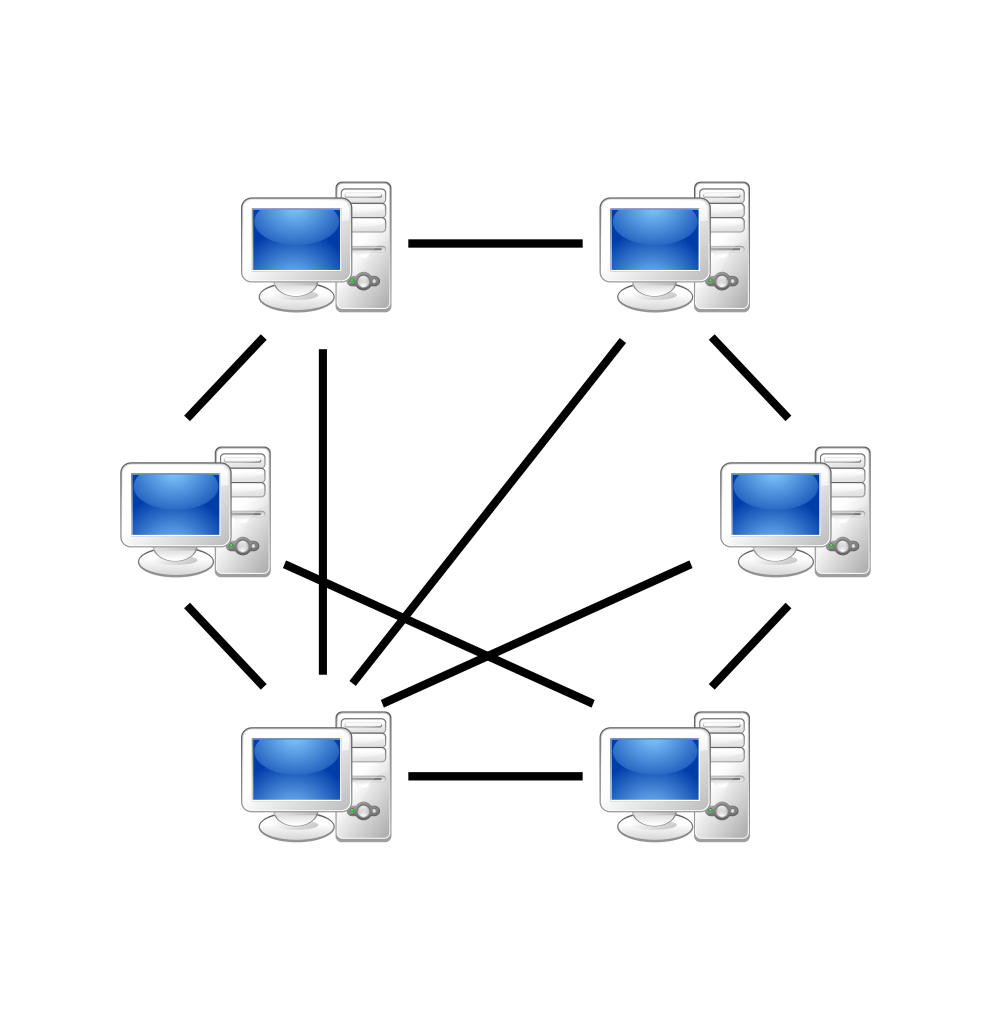
\includegraphics[width=50mm, keepaspectratio]{figures/P2P-network.png}\hspace{1cm}
	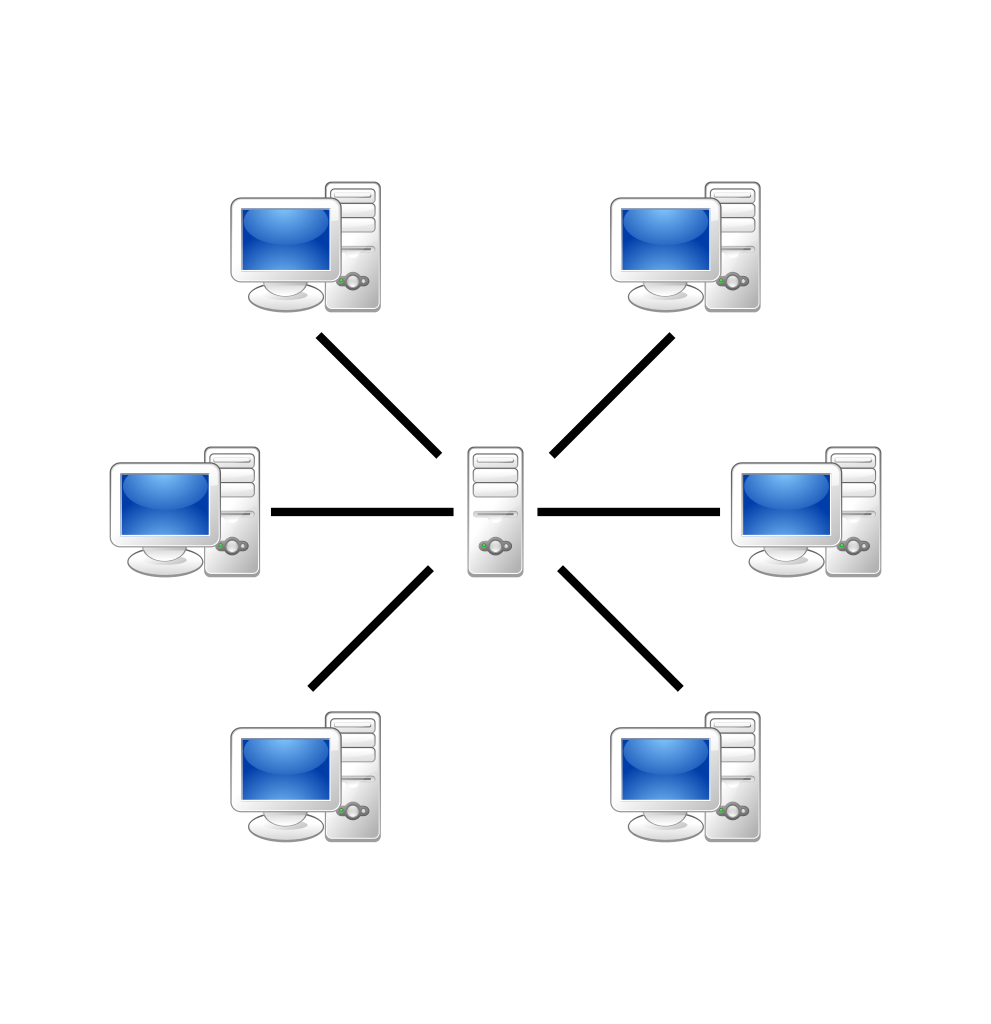
\includegraphics[width=50mm, keepaspectratio]{figures/Server-based-network.png}
	\caption{P2P és kliens-szerver alapú hálózat.}%TODO forrásmegjelölés
	\label{fig:HVSpaces}
\end{figure}

P2P hálózat használatának fő előnye a robusztusság és a skálázhatóság, mivel nincs központi elem,
aminek a meghibásodása szolgáltatáskiesést okozhatna, illetve a hálózat minden tagja hozzájárul a
szolgáltatás minőségének fenntartásához. (pl. P2P alapú fájlmegosztás esetén esetén a letöltés
mellett fel is tölt) Hátrányai közül a két legjelentősebb a nehezebb karbantarthatóság, és az
esetlegesen fellépő sebességproblémák internetszolgáltató-oldali forgalomkorlátozások miatt.
A P2P alapú technológiák egyik legnagyobb felhasználási területe a tartalomszolgáltatás, ezen belül
az egyik legismertebb ilyen technológiát használó protokoll a Bittorrent. A Bittorrent protokollt
fájlmegosztásra használjuk, a mögötte álló alapvető ötlet az, hogy a megosztandó fájlokat
feldaraboljuk, és a letöltőknek ezeket a darabokat nem ugyanolyan sorrendben adjuk oda, így ők a
hiányzó darabokat egymástól is tudják tölteni. 
